\providecommand{\atd}{..}
\documentclass[../main.tex]{subfiles}

\begin{document}
    \chapter{Personas}\label{ch:topic}

    \section{Context}\label{sec:introduction}
    \subsection{Considerations about the selection of our personas}
    In the context of the people’s safety, the Protezione Civile authority occupies the role of one of the city security guarantors. We selected two members of this organization and detailed their activities with the purpose of defining the functional requirements of the solution we are proposing. The subjects are distinguished by a different seniority level and by roles that include activities performed with different levels of abstraction. 
    The primary persona, identified by Giulio Fumagalli, covers the role of supervisor agent in the operative centre of the Italian Civil Protection of Milan. His operational tasks are the starting point for our analysis of the reference context because satisfying his need implies bringing added value also to his operating chief. This is due to the different approaches the two personas have when facing an emerging problem. In fact, Giulio is the person which will interact directly with our system: in the example of managing the Covid-19 pandemic situation Giulio will be able to perform, using the system interface, targeted searches and analysis of people turned out to be infected and the contacts they had. His superior, Luigi D’Angelo, is able to get major improvements in the effectiveness and in the efficiency of his team in performing their task, if they can rely on such a system. The models below detail the described scenario focusing on the users behaviors and activities.



    \section{Primary: Giulio, the tireless worker}\label{sec:primary-persona}
    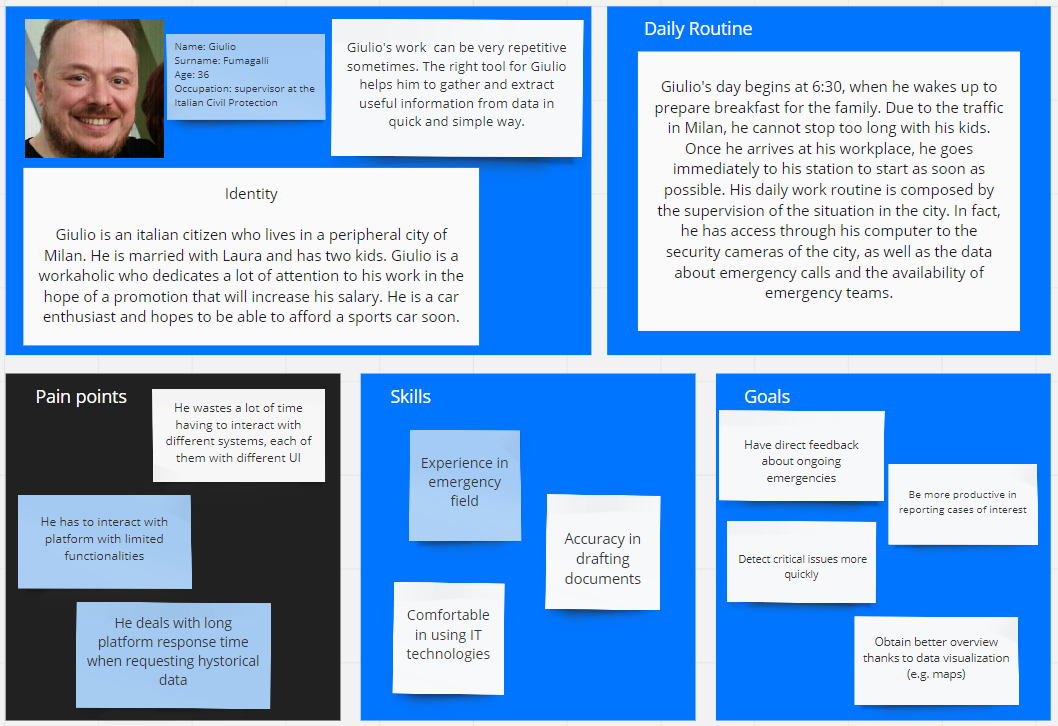
\includegraphics[scale = 0.45]{assets/primary.png}
    \section{Secondary: Luigi, the protective father}\label{sec:secondary-persona}
    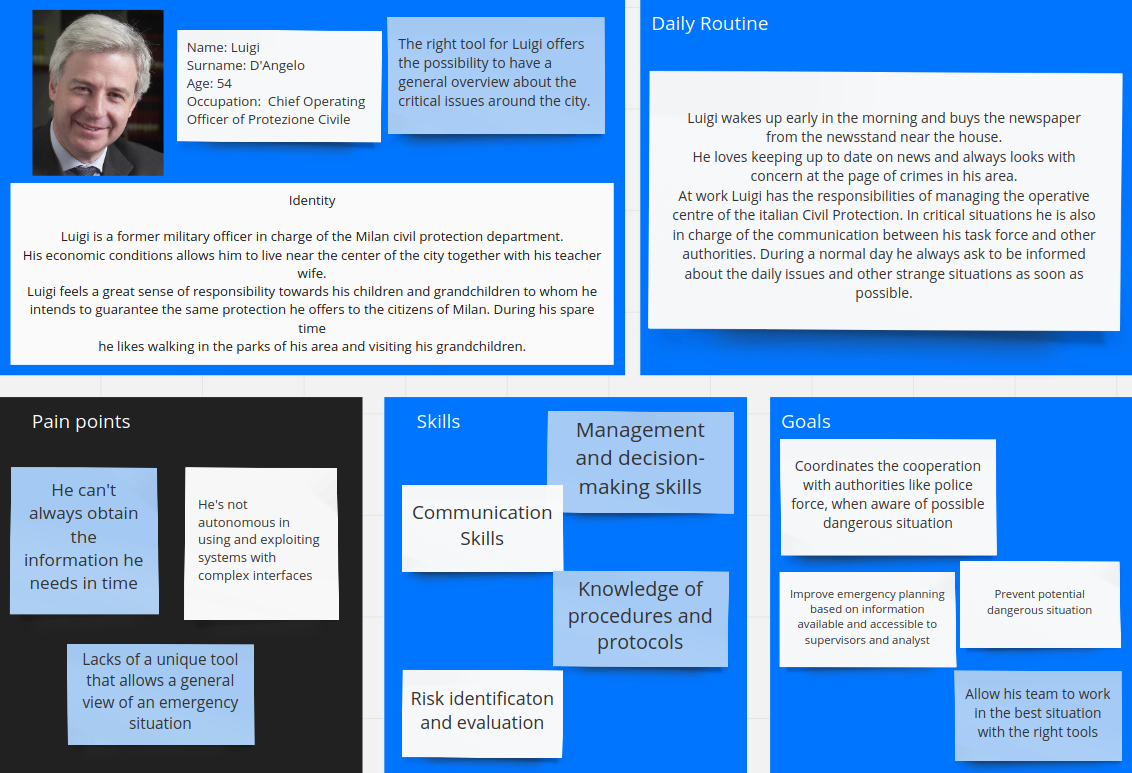
\includegraphics[scale = 0.45]{assets/secondary.png}
    \section{Personas Radar}\label{sec:personas-radar}

    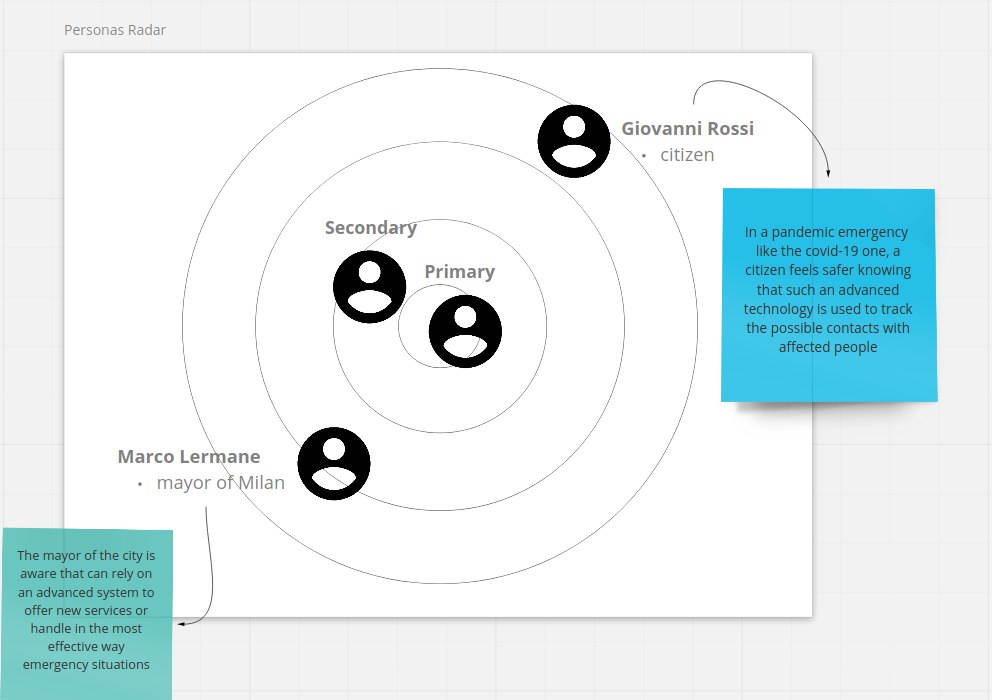
\includegraphics[scale = 0.5]{assets/radar.jpg}

    \chapter{Thinking Hats}\label{ch:thinking-hats}
    \section{Introduction}\label{sec:introduction2}
    Using the 6 hats methodology, we engaged two types of discussion: the “Initial Ideas” and the “Identifying Solutions”. In this way we have been able to support the conversation in 4 people, and also to insert considerations of hats non included in the 2 (like the red hat).
    We used the following person-hat combination for the two rounds:
    \begin{itemize}
        \item Lorenzo Genesi: Yellow - Blue
        \item Gabriel Raul Marini: Blue - Green
        \item Federico Morreale: Green - White
        \item Luigi Pederzani: White - Black
    \end{itemize}
    Plus a round with all the people wearing the same hat, in order to cover all the hats.
    We have created a summary of the main point discussed and presented by each hat following the chronological order of the discussion, highlighting the interaction between them.


    \subsection{Blue Hat}\label{subsec:blue-hat}
    The blue hat has started and closed the conversation, due to his organising role. He started with a question concerning how technology is now used to ensure the public security. Then, when the discussion went on with some ideas, he focused on them, by asking to define the state of the art of the identified technologies. Afterwards, while the idea has started to be more defined, he tried to put the focus on the possible features.
    At the end, he has closed the conversation by stating a final summary: the fact that our idea is something which can be extremely useful in the context of the pandemic situation, but at the same time it is something that can be exploited also in normal situation.


    \subsection{White Hat}\label{subsec:white-hat}
    The white hat, the informative one, has been able to provide answers to the blue one by giving precise information about the state of the art of what is being discussed. In this way other hats have had an informative base on which they could build their ideas. For example he defined the availability of the data sources and how they are now used by authorities. An important statement, which validates the usability of the product, is the fact that authorities in Italy can have access to certain data sources in case of need, and that in the context of tracking Covid-19 affected people a similar approach has been used in South Korea, with an high success rate.

    \subsection{Green Hat}\label{subsec:green-hat}
    The green hat is the one who has proposed the main idea: he put together the problem of people safety in cities (given by the blue hat), with the possibility of exploiting the enormous quantity of possible data sources and the emergency pandemic condition in which we are living. His idea is to use data to track people movements, and in case of pandemic conditions to track possible contacts with affected people. Afterwards his statements were about applying the newest analysis methodologies to the gathered data (other than visualizing and being able to search in a quick and simple way) and also proposed some possible feature implementation.

    \subsection{Black Hat}\label{subsec:black-hat}
    The black hat has been useful to raise possible problems in the creation and utilization in a system like the proposed one. He pointed out the following problems:
    \begin{itemize}
        \item \textit{Accessing the data}: answered by the white hat, by saying that authorities can obtain access to those data and that the nowadays technologies
        implements interfaces that are able to provide those information
        \item \textit{the perception of privacy of the population}: answered by the yellow one, by saying that with the right shrewdness
        it’s possible to maintain people's privacy and make personal data visible only in particular cases.
        Also the red one gave his point of view, by saying that a system like that would also improve their safety: it can be defined like a trade off
        \item \textit{the possibility that authorities don’t want to invest in a system like the proposed one}
    \end{itemize}


    \subsection{Yellow Hat}\label{subsec:yellow-hat}
    The yellow hat has been able to sustain the proposed ideas by pointing out that our project is based on a technology which is already existing, even if it’s used in other environments. He also pushed on the idea that it would be a game changer in a pandemic condition like the Covid-19 one. Then he contrasted the black hat on the possible privacy problems, and tried to encourage the team on the feasibility of the project.

    \subsection{Red Hat}\label{subsec:red-hat}
    And fourthly the red hat has been able to give some statements about improvements in terms of feeling more safe for normal people and citizens, being aware that such a high technology system is used to ensure public security.
    
    \subsection{Conclusions}\label{subsec:conclusions}
    We have found the 6 hat methodologies, with the suggested tracks, very useful since it forces people in a team to play different roles: even a typically cautious person is forced to wear a creative and intuitive hat and vice versa. In this way is possible to engage a controlled and focused discussion on the main idea which will be developed.

    \section{Hats Table}\label{sec:hats-table}
    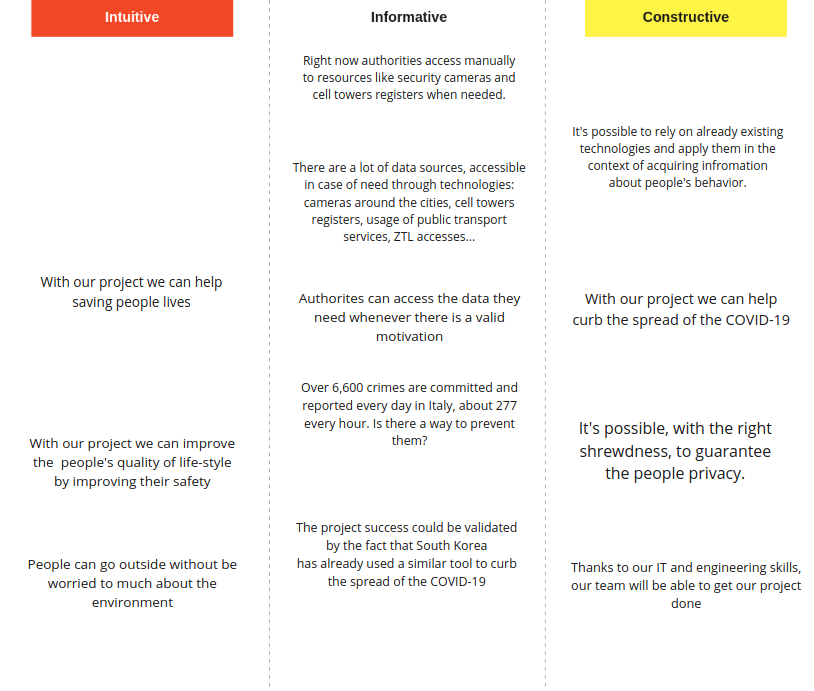
\includegraphics[scale = 0.5]{assets/hat1.png} \\
    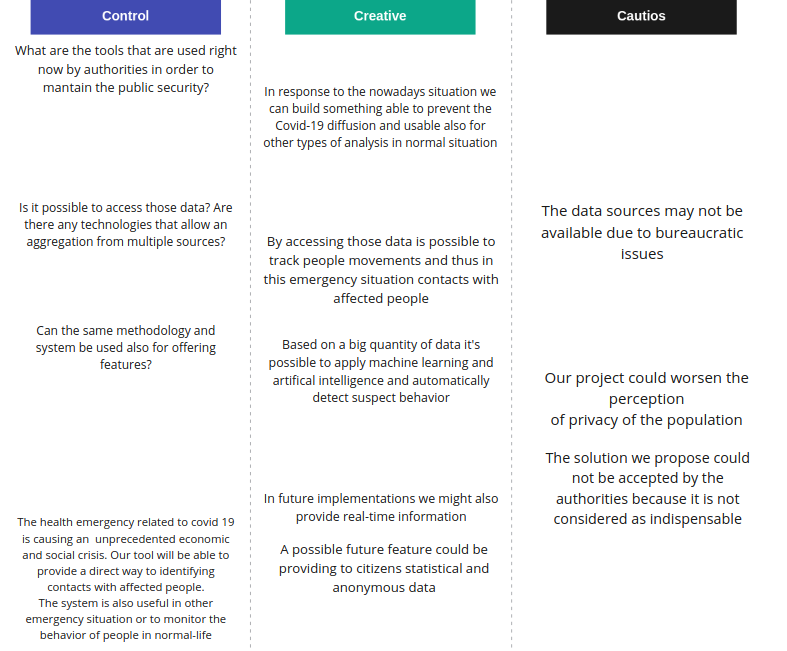
\includegraphics[scale = 0.5]{assets/hat2.png}
\end{document}